\documentclass[11pt,a4paper]{article}

\usepackage[utf8]{inputenc}
\usepackage[T1]{fontenc}
\usepackage{mathpazo}
\usepackage[scaled=0.92]{helvet}
\usepackage[margin=1in]{geometry}
\usepackage{graphicx}
\usepackage{amsmath,amssymb,amsfonts}
\usepackage{booktabs}
\usepackage{tabularx}
\usepackage{setspace}
\usepackage{titlesec}
\usepackage{fancyhdr}
\usepackage{float}
\usepackage{caption}
\usepackage{microtype}
\usepackage{tikz}
\usepackage{xcolor}
\usepackage{listings}
\usepackage[hidelinks]{hyperref}

\usetikzlibrary{shapes.geometric, arrows.meta, positioning, calc, matrix, fit, backgrounds}

\setstretch{1.15}
\setlength{\parindent}{0pt}
\setlength{\parskip}{0.8em}
\sloppy

\titleformat{\section}{\normalfont\large\bfseries\sffamily}{\thesection}{1em}{}
\titleformat{\subsection}{\normalfont\normalsize\bfseries\sffamily}{\thesubsection}{1em}{}
\titleformat{\subsubsection}{\normalfont\normalsize\itshape\sffamily}{\thesubsubsection}{1em}{}

\pagestyle{fancy}
\fancyhf{}
\fancyhead[L]{\small\sffamily Business Analyst Role}
\fancyhead[R]{\small\sffamily\thepage}
\renewcommand{\headrulewidth}{0.4pt}

\captionsetup{font=small,labelfont=bf,labelsep=period}

\renewenvironment{abstract}
{\small
	\begin{center}\textbf{\sffamily Abstrak}\end{center}
	\begin{quote}}
	{\end{quote}}

\lstdefinestyle{code}{
	basicstyle=\ttfamily\small,
	frame=single,
	rulecolor=\color{black},
	breaklines=true,
	showstringspaces=false,
	columns=fullflexible,
	keepspaces=true,
	framesep=6pt,
	aboveskip=1em,
	belowskip=1em,
	xleftmargin=0pt
}

\lstdefinestyle{out}{
	basicstyle=\ttfamily\small,
	frame=tb,
	rulecolor=\color{black},
	breaklines=true,
	showstringspaces=false,
	columns=fullflexible,
	keepspaces=true,
	framesep=4pt,
	aboveskip=1em,
	belowskip=1em
}

\title{\vspace{-1.5cm}\textbf{\sffamily\LARGE Peran Business Analyst\\ dalam Requirement Engineering}}
\author{
	\textbf{Muhammad Riduwan Khafidi} \\
	\small Program Studi Teknik Rekayasa Perangkat Lunak \\
	\small Politeknik Negeri Batam \\
	\small \texttt{4342611034@students.polibatam.ac.id}
}
\date{\small\today}

\begin{document}

\maketitle
\thispagestyle{empty}

\begin{abstract}
	Makalah ini membahas peran Business Analyst dalam requirement engineering dari sudut pandang yang lebih praktis daripada sekadar daftar tanggung jawab. Ia menjelaskan siapa yang disebut analyst, mengapa ia bukan jabatan struktural melainkan peran proyek, apa saja delapan tanggung jawabnya, sembilan skill yang wajib dimiliki, serta tiga latar belakang yang paling sering dipilih menjadi analyst. Tujuh visualisasi dan tiga tabel menyertai pembahasan, termasuk tiga tabel wajib berupa perbandingan ringkasan, kesalahan umum, dan lembar rujukan cepat. Sebuah studi kasus sepuluh langkah menunjukkan artefak konkret yang harus dihasilkan analyst selama satu proyek berjalan. Bagian penutup merangkum tiga prinsip yang membedakan analyst yang efektif dari yang sekadar hadir di rapat.
\end{abstract}

\section{Pendahuluan}

\subsection{Analogi Pembuka}

Bayangkan sebuah orkestra. Ada pemain biola, pemain selo, pemain tiup, dan seorang kondektur. Kondektur tidak memainkan satu alat pun, tapi tanpa dia, setiap pemain akan memainkan tempo dan dinamika versinya sendiri. Kondektur menyatukan mereka menjadi satu suara.

Business Analyst adalah kondektur itu. Ia tidak menulis kode, tapi ia yang memastikan klien, developer, dan manajer berbicara dalam bahasa yang sama sebelum satu nada pun dimainkan.

\subsection{Mengapa Topik Ini Penting}

Pada minggu pertama, kita mempelajari bahwa requirement engineering adalah fondasi seluruh siklus pengembangan. Pada minggu kedua, kita mempelajari bahwa stakeholder tersebar dan tidak selalu sepakat. Di minggu ketiga ini, kita belajar bahwa fondasi dan kesepakatan itu tidak tumbuh sendiri. Ada satu peran yang bertugas menumbuhkannya.

Tanpa analyst, requirement menjadi tumpukan asumsi. Dengan analyst, requirement menjadi dokumen yang bisa diuji dan disepakati.

\subsection{Peta Pembahasan}

Makalah ini disusun berurutan. Bagian kedua menjelaskan siapa Business Analyst dan mengapa ia disebut peran proyek, bukan jabatan. Bagian ketiga membedah delapan tanggung jawabnya. Bagian keempat memetakan sembilan skill yang wajib dimiliki, dibagi menjadi yang bisa dilatih dan yang harus ditumbuhkan. Bagian kelima membandingkan tiga latar belakang yang paling sering menjadi analyst. Bagian keenam membahas konflik dan formula win-win-win. Bagian ketujuh sampai kesembilan merangkum perbandingan, kesalahan umum, dan lembar rujukan cepat. Bagian kesepuluh memandu studi kasus sepuluh langkah, dan bagian kesebelas menutup dengan tiga prinsip.

\section{Siapa Business Analyst}

Requirement Analyst adalah orang yang bertanggung jawab mengumpulkan, menganalisis, mendokumentasikan, dan memvalidasi kebutuhan stakeholder dalam sebuah proyek. Nama lain untuk peran ini antara lain business analyst, requirement engineer, dan requirement manager. Semuanya merujuk pada satu fungsi yang sama.

Yang membedakannya dari jabatan struktural adalah ini: ia adalah \textbf{peran proyek, bukan jabatan}. Siapa pun di dalam proyek bisa ditunjuk memegang peran ini, terlepas dari jabatan formalnya di perusahaan. Seorang developer senior bisa ditunjuk menjadi analyst untuk satu proyek tertentu, sementara jabatan formalnya tetap Software Engineer.

Perhatikan Gambar~\ref{fig:bridge}. Business Analyst adalah jembatan dua arah antara customer dan development team. Arah pertama menerjemahkan kebutuhan bisnis menjadi bahasa teknis. Arah kedua menerjemahkan keterbatasan teknis kembali menjadi bahasa bisnis.

\begin{figure}[H]
	\centering
	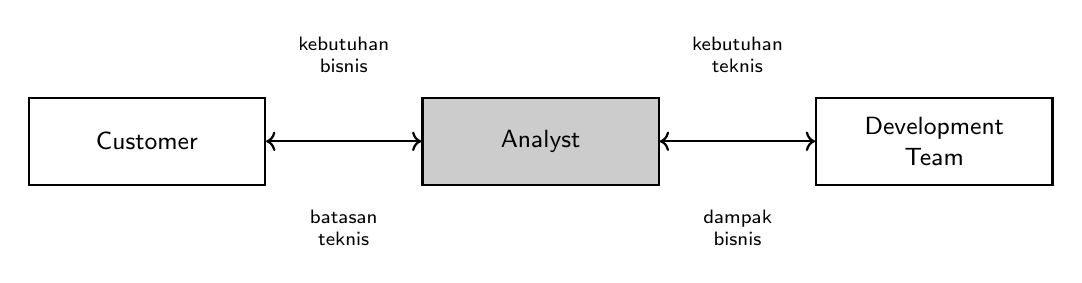
\begin{tikzpicture}[
			bx/.style={rectangle, draw=black, thick, minimum width=3cm, minimum height=1.1cm, align=center, font=\sffamily\small, inner sep=4pt},
			note/.style={font=\sffamily\scriptsize, align=center, text width=2.6cm},
			line/.style={draw, thick, <->}
		]
		\node[bx, fill=white]    (cust) at (-5, 0) {Customer};
		\node[bx, fill=black!20] (ana)  at ( 0, 0) {Analyst};
		\node[bx, fill=white]    (dev)  at ( 5, 0) {Development\\Team};

		\draw[line] (cust.east) -- (ana.west);
		\draw[line] (ana.east)  -- (dev.west);

		\node[note] at (-2.5, 1.1) {kebutuhan\\bisnis};
		\node[note] at ( 2.5, 1.1) {kebutuhan\\teknis};
		\node[note] at (-2.5, -1.1) {batasan\\teknis};
		\node[note] at ( 2.5, -1.1) {dampak\\bisnis};
	\end{tikzpicture}
	\caption{Analyst sebagai jembatan dua arah antara customer dan development team.}
	\label{fig:bridge}
\end{figure}

Kata kunci yang sering terlewat adalah \textbf{dua arah}. Analyst yang baik tidak hanya meneruskan permintaan klien ke developer. Ia juga menyampaikan ke klien bahwa permintaannya membawa konsekuensi teknis tertentu. Kalau hanya satu arah, ia bukan jembatan, ia kurir.

Perhatikan Gambar~\ref{fig:role-vs-title}. Ini memperjelas perbedaan antara jabatan formal dan peran proyek.

\begin{figure}[H]
	\centering
	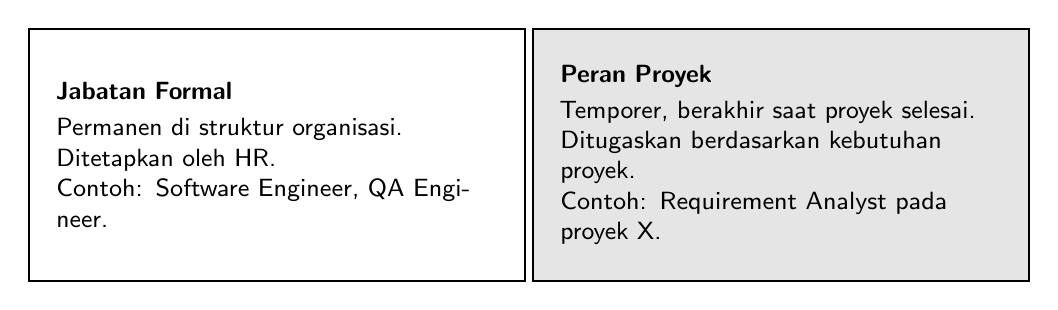
\begin{tikzpicture}[
			rbox/.style={rectangle, draw=black, thick, text width=5.6cm, align=left, font=\sffamily\small, inner sep=10pt, minimum height=3.2cm}
		]
		\node[rbox, fill=white, anchor=north west] (a) at (-6.1, 0) {
			\textbf{Jabatan Formal} \\[2pt]
			Permanen di struktur organisasi. \\
			Ditetapkan oleh HR. \\
			Contoh: Software Engineer, QA Engineer.
		};
		\node[rbox, fill=black!10, anchor=north west] (b) at (0.3, 0) {
			\textbf{Peran Proyek} \\[2pt]
			Temporer, berakhir saat proyek selesai. \\
			Ditugaskan berdasarkan kebutuhan proyek. \\
			Contoh: Requirement Analyst pada proyek X.
		};
	\end{tikzpicture}
	\caption{Perbedaan jabatan formal dan peran proyek.}
	\label{fig:role-vs-title}
\end{figure}

Karena sifatnya peran, bukan jabatan, analyst wajib punya kemampuan, pengetahuan, dan kepribadian yang sesuai. Ia tidak bisa sekadar ``ditunjuk'' tanpa bekal. Bekal itu dibahas pada bagian keempat.

\section{Tanggung Jawab Analyst}

Delapan tanggung jawab berikut membentuk satu siklus penuh. Perhatikan Gambar~\ref{fig:wheel}.

\begin{figure}[H]
	\centering
	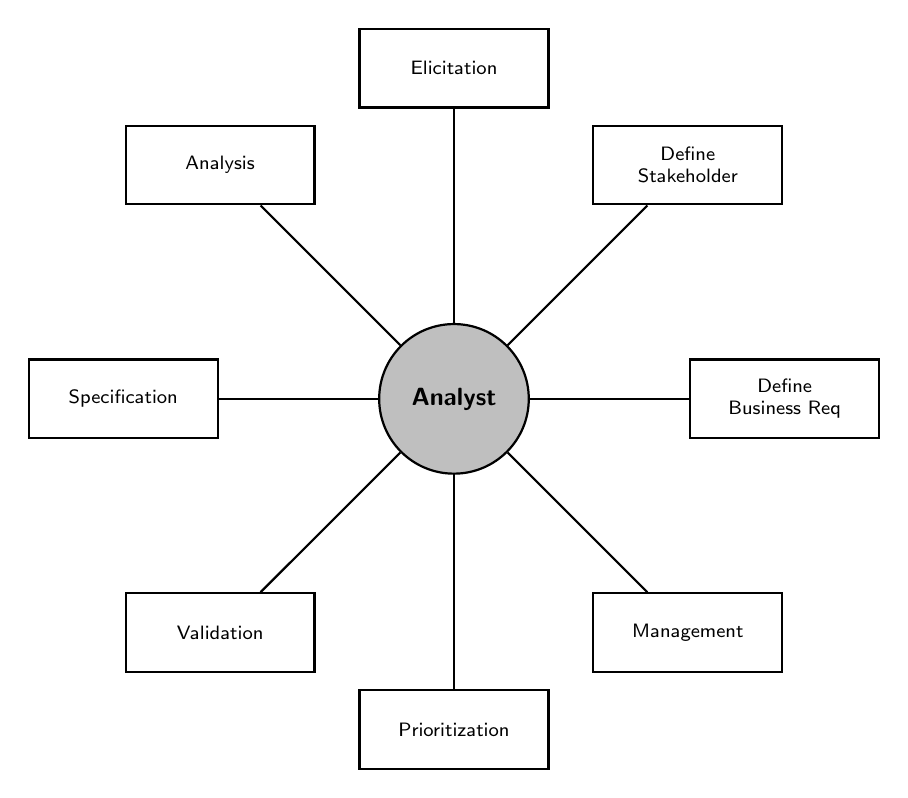
\begin{tikzpicture}[
			hub/.style={circle, draw=black, thick, fill=black!25, minimum size=1.9cm, align=center, font=\sffamily\small\bfseries},
			rbox/.style={rectangle, draw=black, thick, fill=white, minimum width=2.4cm, minimum height=1.0cm, align=center, font=\sffamily\scriptsize, inner sep=3pt},
			line/.style={draw, thick}
		]
		\node[hub] (c) at (0,0) {Analyst};

		\node[rbox] (r1) at ( 4.2,  0)    {Define\\Business Req};
		\node[rbox] (r2) at ( 2.97,  2.97) {Define\\Stakeholder};
		\node[rbox] (r3) at ( 0,     4.2)  {Elicitation};
		\node[rbox] (r4) at (-2.97,  2.97) {Analysis};
		\node[rbox] (r5) at (-4.2,   0)    {Specification};
		\node[rbox] (r6) at (-2.97, -2.97) {Validation};
		\node[rbox] (r7) at ( 0,    -4.2)  {Prioritization};
		\node[rbox] (r8) at ( 2.97, -2.97) {Management};

		\draw[line] (c) -- (r1);
		\draw[line] (c) -- (r2);
		\draw[line] (c) -- (r3);
		\draw[line] (c) -- (r4);
		\draw[line] (c) -- (r5);
		\draw[line] (c) -- (r6);
		\draw[line] (c) -- (r7);
		\draw[line] (c) -- (r8);
	\end{tikzpicture}
	\caption{Delapan tanggung jawab analyst yang membentuk siklus penuh.}
	\label{fig:wheel}
\end{figure}

\textbf{Define business requirement.} Merumuskan alasan mengapa proyek ini ada, apa yang ingin dicapai sponsor, dan batasan yang mengikatnya.

\textbf{Define project stakeholder dan user class.} Mengidentifikasi siapa saja yang terpengaruh, mengelompokkan mereka ke user class, dan menandai mana yang favored.

\textbf{Elicitation.} Menggali kebutuhan secara proaktif. Tekniknya bisa wawancara, workshop, analisis dokumen, kunjungan ke lokasi customer, analisis business process, analisis produk kompetitor, atau reverse engineering sistem yang sudah ada.

\textbf{Analysis.} Memeriksa hasil elicitation. Mencari konflik, kesenjangan, dan asumsi yang belum terverifikasi.

\textbf{Specification.} Menuliskan hasil analisis ke dalam dokumen yang mudah dipahami. Formatnya bisa tabel, persamaan matematika, storyboard, prototipe, atau diagram.

\textbf{Validation.} Memimpin proses konfirmasi dokumen ke stakeholder. Memastikan tidak ada yang kurang, lebih, atau salah tafsir.

\textbf{Prioritization.} Memfasilitasi penentuan prioritas requirement. Analyst tidak memutuskan, tapi memastikan keputusan diambil dengan informasi yang cukup.

\textbf{Management.} Menjaga agar requirement tetap terkendali sepanjang proyek, termasuk melacak perubahan dan mengevaluasi dampaknya sebelum disetujui.

\section{Skill yang Wajib Dimiliki}

Sembilan skill berikut membentuk profil seorang analyst. Perhatikan Gambar~\ref{fig:skills}.

\begin{figure}[H]
	\centering
	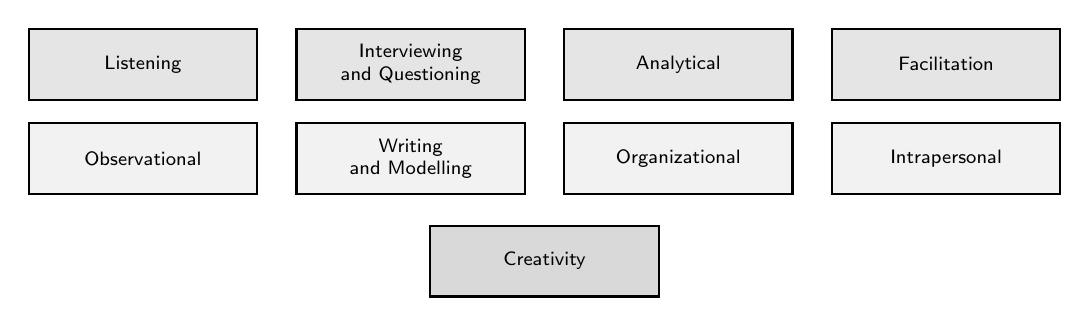
\begin{tikzpicture}[
			skillcard/.style={rectangle, draw=black, thick, minimum width=2.9cm, minimum height=0.9cm, align=center, font=\sffamily\scriptsize, inner sep=3pt}
		]
		\node[skillcard, fill=black!10] (s1) at (-5.1, 1.5) {Listening};
		\node[skillcard, fill=black!10] (s2) at (-1.7, 1.5) {Interviewing\\and Questioning};
		\node[skillcard, fill=black!10] (s3) at ( 1.7, 1.5) {Analytical};
		\node[skillcard, fill=black!10] (s4) at ( 5.1, 1.5) {Facilitation};

		\node[skillcard, fill=black!5] (s5) at (-5.1, 0.3) {Observational};
		\node[skillcard, fill=black!5] (s6) at (-1.7, 0.3) {Writing\\and Modelling};
		\node[skillcard, fill=black!5] (s7) at ( 1.7, 0.3) {Organizational};
		\node[skillcard, fill=black!5] (s8) at ( 5.1, 0.3) {Intrapersonal};

		\node[skillcard, fill=black!15] (s9) at ( 0, -1.0) {Creativity};
	\end{tikzpicture}
	\caption{Sembilan skill esensial seorang analyst.}
	\label{fig:skills}
\end{figure}

Sembilan skill ini tidak dilatih dengan cara yang sama. Sebagian bisa diajarkan lewat pelatihan formal, sebagian lain hanya tumbuh lewat pengalaman. Perhatikan Gambar~\ref{fig:train-vs-grow}.

\begin{figure}[H]
	\centering
	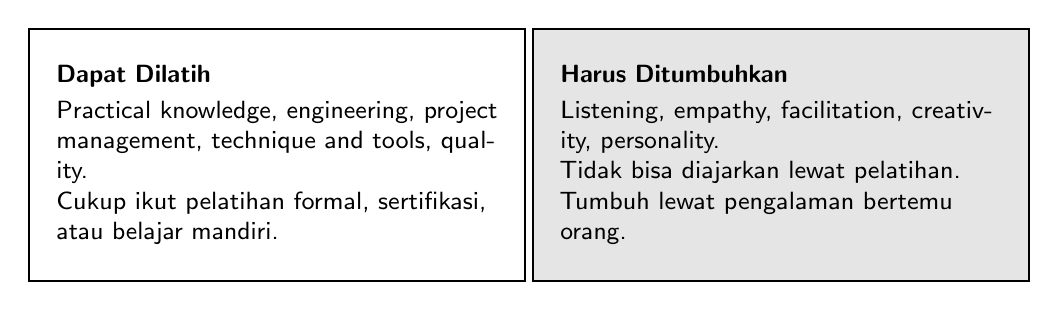
\begin{tikzpicture}[
			tbox/.style={rectangle, draw=black, thick, text width=5.6cm, align=left, font=\sffamily\small, inner sep=10pt, minimum height=3.2cm}
		]
		\node[tbox, fill=white, anchor=north west] (a) at (-6.1, 0) {
			\textbf{Dapat Dilatih} \\[2pt]
			Practical knowledge, engineering, project management, technique and tools, quality. \\
			Cukup ikut pelatihan formal, sertifikasi, atau belajar mandiri.
		};
		\node[tbox, fill=black!10, anchor=north west] (b) at (0.3, 0) {
			\textbf{Harus Ditumbuhkan} \\[2pt]
			Listening, empathy, facilitation, creativity, personality. \\
			Tidak bisa diajarkan lewat pelatihan. Tumbuh lewat pengalaman bertemu orang.
		};
	\end{tikzpicture}
	\caption{Perbedaan skill yang dapat dilatih dan yang harus ditumbuhkan.}
	\label{fig:train-vs-grow}
\end{figure}

Karena itu, kalimat ``good analyst is grown rather than trained'' bukan retorika. Analyst yang baik tidak lahir dari sertifikat, tapi dari ratusan jam wawancara, puluhan workshop yang gagal, dan refleksi dari setiap kegagalan itu.

Tidak ada kurikulum pendidikan standar untuk analyst. Tapi paling tidak, analyst harus punya enam bekal dasar: practical knowledge, engineering, project management, technique and tools, quality, dan personality.

\section{Siapa yang Bisa Menjadi Analyst}

Tiga latar belakang paling sering menjadi analyst. Perhatikan Gambar~\ref{fig:backgrounds}. Masing-masing punya sisi kuat dan sisi lemah yang perlu disadari sejak awal.

\begin{figure}[H]
	\centering
	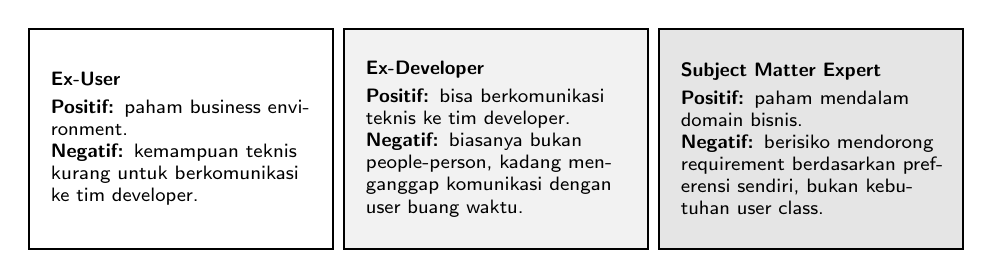
\begin{tikzpicture}[
			candbox/.style={rectangle, draw=black, thick, text width=3.3cm, align=left, font=\sffamily\scriptsize, inner sep=8pt, minimum height=2.8cm}
		]
		\node[candbox, fill=white, anchor=north west] (u) at (-6.3, 0) {
			\textbf{Ex-User} \\[2pt]
			\textbf{Positif:} paham business environment. \\
			\textbf{Negatif:} kemampuan teknis kurang untuk berkomunikasi ke tim developer.
		};
		\node[candbox, fill=black!5, anchor=north west] (d) at (-2.3, 0) {
			\textbf{Ex-Developer} \\[2pt]
			\textbf{Positif:} bisa berkomunikasi teknis ke tim developer. \\
			\textbf{Negatif:} biasanya bukan people-person, kadang menganggap komunikasi dengan user buang waktu.
		};
		\node[candbox, fill=black!10, anchor=north west] (s) at (1.7, 0) {
			\textbf{Subject Matter Expert} \\[2pt]
			\textbf{Positif:} paham mendalam domain bisnis. \\
			\textbf{Negatif:} berisiko mendorong requirement berdasarkan preferensi sendiri, bukan kebutuhan user class.
		};
	\end{tikzpicture}
	\caption{Tiga latar belakang calon analyst beserta kekuatan dan kelemahannya.}
	\label{fig:backgrounds}
\end{figure}

\textbf{Ex-user} membawa pemahaman mendalam tentang bagaimana bisnis berjalan sehari-hari. Kelemahannya, ia sering kesulitan menerjemahkan pemahaman itu ke bahasa teknis yang dimengerti developer.

\textbf{Ex-developer} sudah fasih berbahasa teknis. Kelemahannya, ia cenderung ingin segera masuk ke proses pengembangan dan menganggap komunikasi dengan user sebagai formalitas yang memperlambat.

\textbf{Subject matter expert} menguasai domain lebih dalam dari siapa pun. Kelemahannya, ia berisiko mendorong requirement berdasarkan preferensi pribadinya, bukan berdasarkan kebutuhan seluruh user class.

Tidak ada latar belakang yang unggul secara mutlak. Yang ada adalah latar belakang yang cocok untuk konteks proyek tertentu. Proyek yang domain bisnisnya sangat khusus lebih cocok dipimpin SME. Proyek yang sangat teknis lebih cocok dipimpin ex-developer. Proyek yang penggunanya sangat beragam lebih cocok dipimpin ex-user.

\section{Konflik dan Formula Win-Win-Win}

Di dalam proyek, hubungan antara analyst, developer, user, dan manajer tidak selalu mulus. Masing-masing pihak punya motivasi, kebutuhan, dan batasan yang berbeda. Mereka tidak selalu saling percaya dan menghormati.

Peran analyst bukan memenangkan salah satu pihak. Peran analyst adalah memastikan ketiga pihak menang sekaligus. Perhatikan Gambar~\ref{fig:winwinwin}.

\begin{figure}[H]
	\centering
	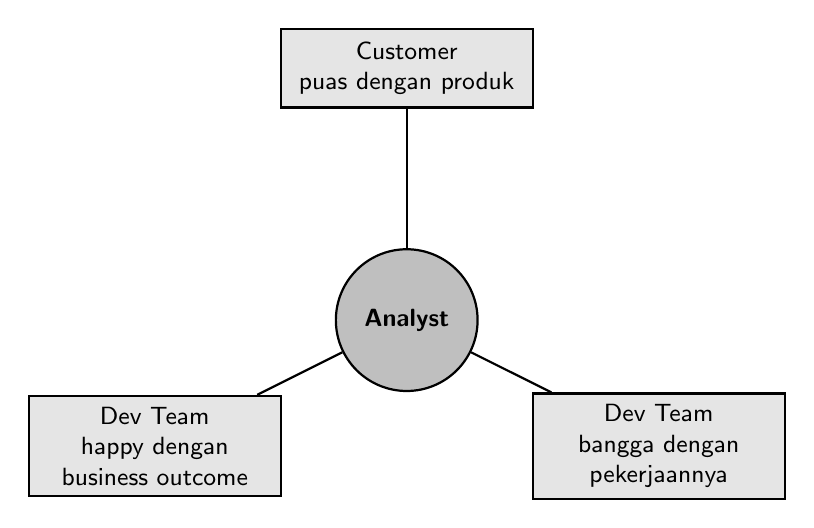
\begin{tikzpicture}[
			winbox/.style={rectangle, draw=black, thick, fill=black!10, minimum width=3.2cm, minimum height=1.0cm, align=center, font=\sffamily\small, inner sep=4pt},
			hub/.style={circle, draw=black, thick, fill=black!25, minimum size=1.8cm, align=center, font=\sffamily\small\bfseries},
			line/.style={draw, thick}
		]
		\node[winbox] (cust) at ( 0,    3.2) {Customer\\puas dengan produk};
		\node[winbox] (biz)  at (-3.2, -1.6) {Dev Team\\happy dengan\\business outcome};
		\node[winbox] (work) at ( 3.2, -1.6) {Dev Team\\bangga dengan\\pekerjaannya};

		\node[hub] (ana) at (0, 0) {Analyst};

		\draw[line] (ana) -- (cust);
		\draw[line] (ana) -- (biz);
		\draw[line] (ana) -- (work);
	\end{tikzpicture}
	\caption{Analyst menjamin tiga kepuasan sekaligus.}
	\label{fig:winwinwin}
\end{figure}

Tiga pihak yang harus menang:

\textbf{Pertama, customer puas dengan produk yang dikirim.} Bukan hanya sesuai spesifikasi, tapi benar-benar menyelesaikan masalah yang dihadapi.

\textbf{Kedua, development team senang dengan business outcome.} Bukan hanya karena proyek selesai, tapi karena hasilnya punya dampak nyata.

\textbf{Ketiga, development team bangga dengan pekerjaannya.} Bukan hanya karena dibayar, tapi karena proyeknya menantang dan memberi ruang bertumbuh.

Tiga kepuasan ini tidak saling meniadakan. Analyst yang baik tidak mengorbankan satu pihak untuk memuaskan pihak lain. Ia mencari titik di mana ketiganya bisa terpenuhi. Itulah esensi win-win-win: bukan kompromi, tapi perluasan.

\section{Perbandingan Ringkasan}

Tabel~\ref{tab:summary} merangkum perbedaan kunci yang telah dibahas.

\begin{table}[H]
	\centering
	\caption{Ringkasan konsep utama minggu ketiga.}
	\label{tab:summary}
	\footnotesize
	\begin{tabularx}{\textwidth}{l X X}
		\toprule
		Aspek           & Konsep Pertama                    & Konsep Kedua                           \\
		\midrule
		Sifat peran     & Jabatan formal (permanen)         & Peran proyek (temporer)                \\
		Arah komunikasi & Meneruskan kebutuhan ke developer & Menyampaikan dampak teknis ke customer \\
		Jenis skill     & Dapat dilatih (teknis)            & Harus ditumbuhkan (people-oriented)    \\
		Latar belakang  & Ex-developer (kuat teknis)        & Ex-user (kuat domain)                  \\
		Formula hasil   & Menang satu pihak                 & Win-win-win untuk tiga pihak           \\
		Fokus analyst   & Memutuskan prioritas              & Memfasilitasi keputusan prioritas      \\
		\bottomrule
	\end{tabularx}
\end{table}

\section{Studi Kasus: Sepuluh Langkah Menjalankan Peran Analyst}

Bagian ini memandu langkah demi langkah untuk mempraktikkan peran analyst dalam satu proyek. Contoh kasus: Sistem Manajemen Inventori untuk sebuah toko ritel kecil. Setiap langkah menghasilkan satu artefak konkret.

\subsection{Langkah 1: Petakan Peran dan Tanggung Jawab}

Sebelum bertindak, tulis dulu apa yang akan dan tidak akan dilakukan.

\begin{lstlisting}[style=out]
Peran Analyst dalam Proyek Ini:

Akan dilakukan:
- Memimpin wawancara dengan pemilik toko
- Menyusun dokumen requirement
- Memfasilitasi prioritisasi
- Mengelola perubahan requirement

Tidak akan dilakukan:
- Menulis kode
- Memutuskan prioritas sendiri
- Menandatangani kontrak
- Mewakili pemilik toko dalam rapat manajemen

Alasan pembatasan:
- Analyst memfasilitasi, bukan mengambil alih
- Keputusan bisnis tetap di tangan sponsor
\end{lstlisting}

\subsection{Langkah 2: Identifikasi Stakeholder dan User Class}

Gunakan tabel dua kolom untuk memisahkan keduanya.

\begin{lstlisting}[style=out]
Stakeholder:
1. Pemilik toko (project sponsor)
2. Kasir (end user)
3. Admin gudang (end user)
4. Supplier (pihak eksternal terdampak)

User Class:
- Kasir (favored) - memakai sistem tiap hari
- Admin gudang (favored) - memakai untuk stok
- Pemilik toko (supporting) - memakai untuk laporan
- Supplier (supporting) - menerima dokumen dari sistem
\end{lstlisting}

\subsection{Langkah 3: Rencanakan Elicitation Multi-Sumber}

Wajib pakai minimal tiga teknik berbeda.

\begin{lstlisting}[style=out]
Rencana Elicitation:

Teknik 1 - Wawancara:
- Pemilik toko, 90 menit, topik visi dan target
- Kasir, 45 menit, topik alur kerja harian

Teknik 2 - Observasi:
- Duduk di samping kasir selama 1 hari kerja
- Catat semua yang kasir lakukan tanpa bertanya

Teknik 3 - Analisis Dokumen:
- Kumpulkan buku catatan stok manual 3 bulan terakhir
- Kumpulkan struk penjualan 1 minggu terakhir
- Identifikasi pola dan anomali
\end{lstlisting}

\subsection{Langkah 4: Catat Temuan Elicitation Secara Real-Time}

Tulis saat wawancara berlangsung, bukan setelahnya.

\begin{lstlisting}[style=out]
Catatan Lapangan 1 (Wawancara Kasir):

Kasir bilang: "Kalau stok habis, saya harus telepon
gudang dulu. Kadang gudang baru tahu besok paginya."

Interpretasi analyst (BELUM dikonfirmasi):
- Mungkin butuh fitur notifikasi otomatis ke gudang
- Mungkin butuh fitur cek stok real-time

Tindak lanjut:
- Konfirmasi ke admin gudang apakah notifikasi
  via aplikasi atau SMS lebih cocok
\end{lstlisting}

\subsection{Langkah 5: Analisis Konflik dan Kesenjangan}

Setelah semua data terkumpul, periksa benturan antar kebutuhan.

\begin{lstlisting}[style=out]
Analisis Konflik:

Konflik 1:
- Kasir ingin cek stok cepat (di bawah 3 detik)
- Admin gudang ingin update stok segera setelah
  barang keluar

Solusi:
- Buat dua tampilan berbeda: satu untuk kasir
  (read-only, cepat), satu untuk admin (write,
  dengan konfirmasi)

Kesenjangan:
- Tidak ada yang menyebut siapa yang menangani
  selisih stok fisik vs catatan sistem
- Harus dikonfirmasi ke pemilik toko sebelum
  spesifikasi ditulis
\end{lstlisting}

\subsection{Langkah 6: Tulis Spesifikasi Requirement}

Ubah temuan menjadi requirement yang bisa diuji.

\begin{lstlisting}[style=out]
FR-01: Kasir melihat stok terkini dalam waktu
kurang dari 3 detik setelah membuka layar.
Input: kode barang.
Output: nama, jumlah stok, satuan.

FR-02: Admin gudang memperbarui stok dengan
konfirmasi ganda.
Input: kode barang, jumlah baru, alasan perubahan.
Output: catatan perubahan stok dengan timestamp
dan nama admin.

NFR-01: Sistem menangani minimal 50 transaksi
per menit pada jam sibuk.

NFR-02: Data stok tersinkronisasi ke cadangan
setiap 10 menit.
\end{lstlisting}

\subsection{Langkah 7: Fasilitasi Prioritisasi}

Analyst tidak memutuskan, tapi memandu keputusan.

\begin{lstlisting}[style=out]
Agenda Prioritisasi dengan Sponsor:

Metode: MoSCoW (Must, Should, Could, Won't)

Harus ada di rilis pertama:
- FR-01 (lihat stok cepat) - kritis untuk kasir
- FR-02 (update stok) - kritis untuk gudang

Sebaiknya ada di rilis pertama:
- Laporan stok mingguan ke pemilik

Bisa ditunda:
- Notifikasi otomatis ke gudang

Tidak akan dikerjakan di rilis ini:
- Integrasi dengan sistem akuntansi eksternal

Keputusan diambil oleh: sponsor
Analyst mencatat dan mendokumentasikan
\end{lstlisting}

\subsection{Langkah 8: Pimpin Validasi}

Bukan sekadar presentasi, tapi konfirmasi dua arah.

\begin{lstlisting}[style=out]
Agenda Validasi:

Sesi 1 - dengan Kasir (30 menit):
- Demonstrasi prototipe layar cek stok
- Minta kasir coba 5 skenario berbeda
- Catat semua ketidaknyamanan

Sesi 2 - dengan Admin Gudang (45 menit):
- Demonstrasi alur update stok
- Uji skenario konflik: dua admin update
  barang yang sama bersamaan

Sesi 3 - dengan Sponsor (60 menit):
- Presentasi dokumen requirement final
- Konfirmasi scope dan out-of-scope
- Tanda tangan persetujuan

Kriteria validasi:
- Semua stakeholder favored hadir di sesinya
- Setiap requirement sudah diuji dengan data nyata
- Tidak ada requirement yang masih ambigu
\end{lstlisting}

\subsection{Langkah 9: Kelola Perubahan}

Setelah dokumen disahkan, kunci dan kelola perubahannya.

\begin{lstlisting}[style=out]
Prosedur Change Request:

Setiap usulan perubahan harus melalui:

1. Formulir CR berisi: deskripsi, alasan, dampak
   ke jadwal, dampak ke anggaran
2. Analyst mengevaluasi dampak teknis dan
   dampak ke requirement lain
3. Sponsor memutuskan: terima, tolak, atau
   jadwalkan untuk rilis berikutnya
4. Jika diterima, dokumen diperbarui dan
   versi baru diterbitkan
5. Semua CR dicatat di change log

Aturan penutup:
- Tidak ada perubahan tanpa formulir
- Tidak ada keputusan tanpa sponsor
- Tidak ada versi tanpa catatan perubahan
\end{lstlisting}

\subsection{Langkah 10: Refleksi Peran}

Di akhir proyek, evaluasi apakah peran dijalankan dengan benar.

\begin{lstlisting}[style=out]
Refleksi Akhir Proyek:

Yang berjalan baik:
- Kasir dan admin gudang puas dengan produk
- Tidak ada requirement yang berubah setelah
  tanda tangan sponsor

Yang perlu diperbaiki:
- Wawancara awal terlalu singkat (45 menit)
- Seharusnya observasi dilakukan lebih awal,
  sebelum wawancara, agar pertanyaan lebih tajam

Pelajaran untuk proyek berikutnya:
- Alokasi waktu: 60 persen mendengar, 30 persen
  bertanya, 10 persen menulis. Bukan sebaliknya.
\end{lstlisting}

Sepuluh langkah di atas menghasilkan empat artefak siap kumpul: dokumen peran dan tanggung jawab, dokumen requirement hasil elicitation, catatan prioritisasi dan validasi, serta catatan refleksi akhir proyek. Inilah deliverable minggu ketiga.

\section{Kesalahan Umum}

Tabel~\ref{tab:mistakes} merangkum kesalahan yang paling sering dilakukan analyst pemula.

\begin{table}[H]
	\centering
	\caption{Kesalahan umum pada peran Business Analyst.}
	\label{tab:mistakes}
	\footnotesize
	\begin{tabularx}{\textwidth}{l X X}
		\toprule
		Kesalahan                                       & Akibat                                    & Perbaikan                                                    \\
		\midrule
		Menganggap analyst sebagai jabatan, bukan peran & Salah menilai siapa yang berhak ditunjuk  & Pahami bahwa peran bisa dipegang siapa pun di proyek         \\
		Meneruskan permintaan klien tanpa menerjemahkan & Developer menerima requirement mentah     & Terjemahkan dulu ke bahasa teknis, konfirmasi balik ke klien \\
		Hanya mendengar satu arah                       & Kebutuhan klien tidak dikontekstualisasi  & Selalu sampaikan dampak teknis ke klien                      \\
		Mengambil keputusan prioritas sendiri           & Keputusan bisnis diambil pihak yang salah & Fasilitasi keputusan, jangan mengambil alih                  \\
		Elicitation hanya lewat wawancara               & Gambaran tidak lengkap                    & Gabungkan minimal tiga teknik                                \\
		Mencatat temuan setelah wawancara selesai       & Detail penting hilang                     & Catat sambil berlangsung, verifikasi ke narasumber           \\
		Melewatkan analisis konflik                     & Requirement bertentangan lolos ke dokumen & Lakukan analisis eksplisit sebelum menulis spesifikasi       \\
		Menganggap validasi sebagai presentasi          & Stakeholder belum benar-benar setuju      & Minta uji coba prototipe dan tanda tangan                    \\
		\bottomrule
	\end{tabularx}
\end{table}

Tiga kesalahan yang paling sering terjadi adalah \textbf{mengambil keputusan prioritas sendiri}, \textbf{meneruskan permintaan klien tanpa menerjemahkan}, dan \textbf{mencatat temuan setelah wawancara selesai}. Ketiganya berakar pada satu hal yang sama: analyst merasa dirinya harus produktif dengan bertindak cepat, padahal nilai analyst justru pada ketelitian dan kesabarannya.

\section{Lembar Rujukan Cepat}

Tabel~\ref{tab:cheat} adalah ringkasan istilah dan artefak yang wajib dikuasai sebelum pertemuan keempat.

\begin{table}[H]
	\centering
	\caption{Lembar rujukan cepat untuk minggu ketiga.}
	\label{tab:cheat}
	\footnotesize
	\begin{tabularx}{\textwidth}{l X}
		\toprule
		Kebutuhan atau Istilah      & Definisi atau Artefak                                                        \\
		\midrule
		Business Analyst            & Peran yang mengumpulkan, menganalisis, dan memvalidasi kebutuhan stakeholder \\
		Requirement Analyst         & Nama lain untuk peran yang sama                                              \\
		Requirement Engineer        & Nama lain untuk peran yang sama                                              \\
		Requirement Manager         & Nama lain untuk peran yang sama                                              \\
		Peran proyek                & Temporer, ditugaskan berdasarkan kebutuhan proyek, bukan jabatan HR          \\
		Jabatan formal              & Permanen, ditetapkan HR, tidak berakhir saat proyek selesai                  \\
		Define business requirement & Merumuskan alasan proyek dan target sponsor                                  \\
		Define stakeholder          & Mengidentifikasi pihak yang terpengaruh                                      \\
		Elicitation                 & Menggali kebutuhan lewat wawancara, observasi, dokumen, workshop             \\
		Analysis                    & Memeriksa konflik, kesenjangan, dan asumsi                                   \\
		Specification               & Menulis requirement dalam format yang bisa diuji                             \\
		Validation                  & Konfirmasi dua arah ke stakeholder                                           \\
		Prioritization              & Memfasilitasi keputusan prioritas, bukan mengambil alih                      \\
		Management                  & Tracking perubahan dan mengevaluasi dampaknya                                \\
		Win-win-win                 & Tiga pihak puas: customer, dev bisnis, dev pekerjaan                         \\
		MoSCoW                      & Metode prioritisasi: Must, Should, Could, Won't                              \\
		\bottomrule
	\end{tabularx}
\end{table}

\section{Kesimpulan}

Business Analyst adalah peran proyek, bukan jabatan formal. Ia menjembatani customer dan development team secara dua arah, mengumpulkan dan memvalidasi kebutuhan, serta menjamin tiga pihak puas sekaligus. Tiga prinsip penutup:

\begin{enumerate}
	\item \textbf{Fasilitasi, jangan ambil alih.} Analyst yang baik memandu keputusan, bukan mengambil keputusan. Prioritas tetap milik sponsor, spesifikasi teknis tetap milik developer. Analyst memastikan keduanya bertemu di titik yang jelas.
	\item \textbf{Sembilan skill, dua cara tumbuh.} Skill teknis bisa dilatih lewat sertifikasi dan pelatihan. Skill people-oriented seperti listening, empathy, dan facilitation hanya tumbuh lewat pengalaman. Kalau hanya fokus pada yang pertama, analyst akan menjadi administrator dokumen, bukan arsitek pemahaman.
	\item \textbf{Catat sambil berjalan.} Ingatan menguap dalam hitungan jam. Analyst yang menulis temuan saat wawancara berlangsung menghasilkan dokumen yang jauh lebih jujur daripada yang merangkum seminggu kemudian. Ini bukan soal disiplin, ini soal menghargai data yang sudah susah payah dikumpulkan.
\end{enumerate}

Pada pertemuan berikutnya, prinsip-prinsip ini akan dipakai untuk mempelajari tipe-tipe requirement secara lebih mendalam. Lembar rujukan cepat di atas adalah bekal minimum yang harus dibawa.

\newpage
\section*{Referensi}
\addcontentsline{toc}{section}{Referensi}

\begin{thebibliography}{99}

	\bibitem{sommerville}
	Sommerville, I. (2016).
	\textit{Software Engineering} (10th ed.).
	Pearson.

	\bibitem{wiegers}
	Wiegers, K., \& Beatty, J. (2013).
	\textit{Software Requirements} (3rd ed.).
	Microsoft Press.

	\bibitem{robertson}
	Robertson, S., \& Robertson, J. (2012).
	\textit{Mastering the Requirements Process: Getting Requirements Right} (3rd ed.).
	Addison-Wesley.

	\bibitem{iiba}
	International Institute of Business Analysis. (2015).
	\textit{A Guide to the Business Analysis Body of Knowledge (BABOK Guide)} (v3.0).
	IIBA.

	\bibitem{podeswa}
	Podeswa, H. (2008).
	\textit{The Business Analyst's Handbook}.
	Course Technology PTR.

	\bibitem{cooke}
	Cooke, J. L. (2013).
	\textit{The Power of the Agile Business Analyst: 30 Surprising Ways a Business Analyst Can Add Value to Your Agile Development Team}.
	IT Governance Publishing.

	\bibitem{hass}
	Hass, K. B. (2011).
	\textit{The Enterprise Business Analyst}.
	Berrett-Koehler Publishers.

	\bibitem{pressman}
	Pressman, R. S., \& Maxim, B. R. (2020).
	\textit{Software Engineering: A Practitioner's Approach} (9th ed.).
	McGraw-Hill Education.

\end{thebibliography}

\end{document}
